\chapter{Design}

For the initial implementation, a single Android app was chosen to test. Despite
this, the library should be generic enough to easily integrate into any Android
application.

There are two core problems to solve. One is finding the best way to capture
enough data from many users' interactions with the application and present it in
a way that will highlight issues in the user interface. The second is keeping
the participants engaged long enough to complete the testing, while using still
the application in a natural way.

Due to the crowdsourced nature of the system, and the fact that no member of the
development team will be present during the testing, the ``think aloud'' aspect
of traditional testing will be missing. It would, of course, be possible to
record the subject speaking as they navigate the application, but it would not
be feasible to collect and aggregate that data automatically from many
participants. Otherwise, the system will incorporate the same ideas as
traditional usability testing.

\section{User Facing Design}

On starting the testing, the user is shown a screen explaining how the testing
will work. They are then presented with a scenario/task for them to complete. On
completion of the task, they will be either given a successive task, or a screen
thanking them for participating. Since multiple tasks would usually be presented to the user in a normal testing session, the developer is able to group tasks together to be performed successively. They are also able to control whether a task follows on from the previous one, or whether they all begin from a common screen. This will be useful for most tasks, where, for example, the developer wants the user to start from a specific screen such as the home screen of the application.

\subsection{Early Versions and Gamification}

In an attempt to keep the user being tested engaged, and thus increasing the likelihood they would complete more of the testing, a game aspect of the framework was considered. In early
iterations the participant could score points by completing tasks. During a task an overlay would show how long the user is taking (\emph{Figure~\ref{fig:initial-overlay}}) and on completion of the task
they would be assigned a number of points relative to how quickly they did it.
Early evaluation of this prototype highlighted a couple of concerns with this approach. Firstly, showing the user how
long they are taking and encouraging them to complete the task as quickly as
possible could cause the participant to focus on the on screen timer instead of other elements of the interface, resulting in behaviour that did not necessarily match real world usage.
Additionally, the point system did not seem to work as hoped, missing crucial aspects that usually make point systems encouraging.  Since the "game" was not really repeatable, and points were not ranked against any other player or used for any other purpose, participants did not see the point (HA I AM SO FUNNY) in gathering them. 

\begin{figure}[ht!]
  \centering 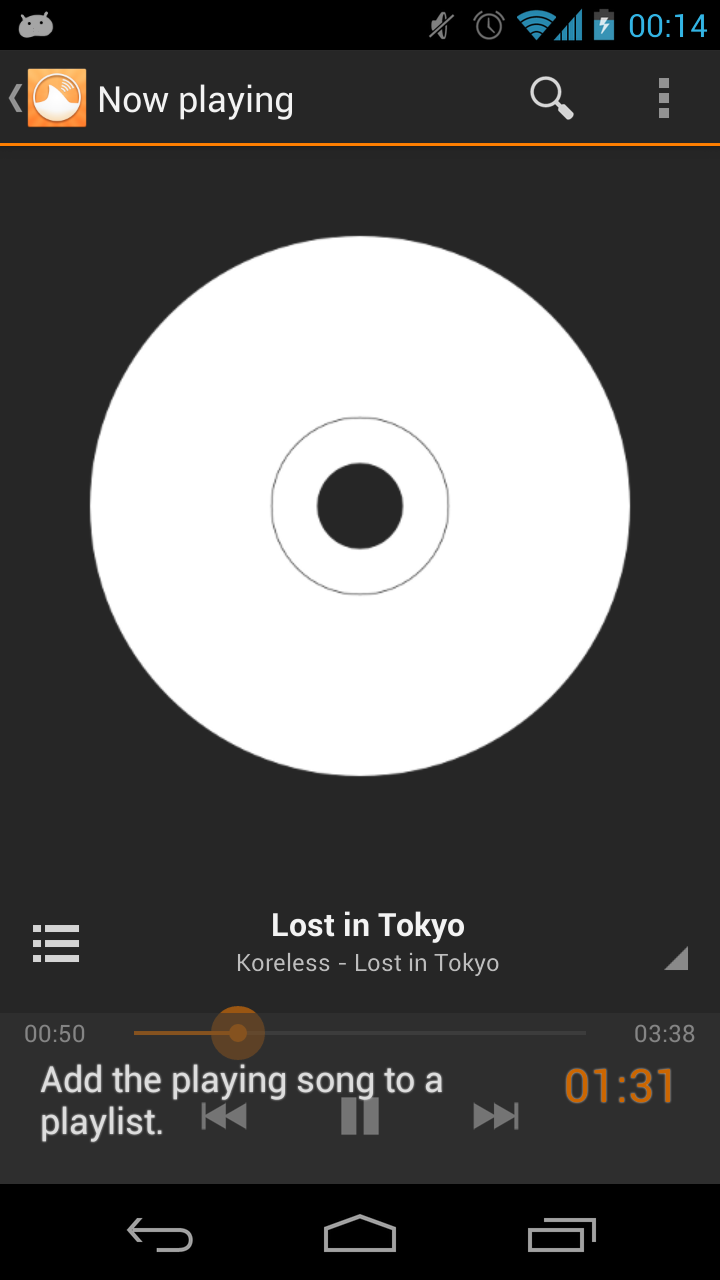
\includegraphics[width=0.5\textwidth]{images/time-taken}
  \caption{The task overlay in early iterations of the project.}
  \label{fig:initial-overlay}
\end{figure}

\todo{Work out what I'm actually doing}
In the current iteration, the thank you screen will also show the user's
``tester rank'', which will depend on the amount of testing that they have
completed compared with the number of tasks/sequences of tasks that are
available within the application. This ranking will encourage the user to
continue participating in the testing, and also allows for rewards (such as
unlocking easter eggs or additional features within the app) if the developer
wishes to include them.

\subsection{In-task UI}

\emph{Figure \ref{fig:initial-overlay}} also shows how the early version of the in-task UI was an overlay over the application interface. While this was semi-transparent, it still had a tendency to obscure important controls, making it harder to use the application. This was refined after the initial evaluation so it no longer obscures content while still displaying important information about the task. The final UI can be seen in \emph{Figure \ref{fig:final-task-overlay}}. While placing an extra piece of interface at the top of the screen will affect the height available to the application, this should not matter since android apps must adapt to different screen sizes anyway, and the space taken up is designed to be as small as possible. Using this design also enables controls to be placed in the in-task UI, here used for an "Abandon" button.

\begin{figure}
  \missingfigure{Show the new in-task UI}
  \label{fig:final-task-overlay}
\end{figure}

\subsection{Abandoning Tasks}

It's likely that for some tasks, a participant might get stuck, and not be able
to complete it. In these cases it seems unfair to penalise them, since the
interface could be too unintuitive or confusing. Worse, this is usually the case
where the developer could benefit most from the feedback, and if the participant
were penalised it could discourage them from continuing with the testing. To
combat this, as part of the overlay that appears while performing a task a
button allows the participant to abandon the current task at any point. This allows the participant to easily continue the testing, and if many people abandon the same task provides a quick indication of tasks that may be especially difficult to complete.

\section{Developer feedback}

To be an effective form of feedback, the system also needs a way for the developer to view the data gathered and identify issues.

There are a few important considerations that need to be made when designing this:

\begin{itemize}
  \item The developer should be able to see as much of the data gathered as possible.
  \item The aggregate performances of many users are far more important than the performance of individual users.
  \item Problem areas within a task should be easy to spot.
  \item Even bigger issues such as tasks that are commonly abandoned should be easy to spot.
\end{itemize}

Some of these criteria are satisfied easily, for example by highlighting tasks with a success rate lower than a certain percentage. To provide a better insight into how people actually attempt to perform a task an interface was developed to show participants navigations through the app during a task (\emph{Figure \ref{fig:task-navigation}}. This interface shows a tree-style view of all the paths that participants took before either completing or abandoning a task. Each branch shows the percentage of users that took that path, allowing the developer can view the most common decisions that users made, and whether they match up to the behaviour that the developer expects.   

\begin{figure}
 \missingfigure{Task navigation tree}
 \label{fig:task-navigation}
\end{figure}



